\section*{Tempo Results}
\addcontentsline{toc}{chapter}{Tempo Results}
\subsection*{Participants}
Five participants (1 male), aged 19-36, with normal hearing and no history of brain injury took part in this study. Four participants had formal musical training (1- 26 years), but none of the participants played instruments regularly at the time of data collection.

\subsection*{Analysis of Beat and Bar-Aligned ERPs}

We analyzed the music stimuli with the dynamic beat tracker \cite{Ellis2007beat} provided by the \emph{librosa} library.\footnote{%
\url{https://github.com/bmcfee/librosa}}
This way, we obtained an estimation of the average tempo as well as annotations for all beats. % (TOTAL NUMBER).
The quality of these automatic annotations was verified through sonification.

Given the beat annotations of the stimuli and assuming that our participants would imagine the stimuli at a similar tempo, 
%we extracted epochs 
%aligned to each beat (excluding cue clicks) and to each bar.
%This resulted in a total of 4x1835 per participant beat-aligned epochs starting XXXms before and ending XXXms after each beat annotation. 
%TODO: timing
%The grand averages are shown in \autoref{fig:beat-aligned grand average} separated by condition.
%TODO: Figure. What can we see? N100? More blurring expected for imagination conditions.
%Maybe, this could be used to develop a beat-detection algorithm -- but we leave this possibility for future work.
%For the bar-aligned ERPs, 
we computed bar-aligned ERPs using non-overlapping epochs from 100ms before to 2.4s after a downbeat annotation.
This length was required to capture slightly more than a single bar for the slowest stimulus -- number 23 with a bar length of more than 2.3s.
As expected, the resulting averaged ERPs differ considerably between participants, stimuli, and conditions.
However, we often observed a periodicity in the averaged signal proportional to the bar length.
%
\autoref{fig:non-overlap_bar-aligned-ERPs} shows example ERPs 
%resulting from averaging non-overlapping epochs from 100ms before to 2.4s after a downbeat annotation.
for a specific participant and stimulus where this is clearly visible in all conditions.

\begin{figure}[t]
  \begin{center}
    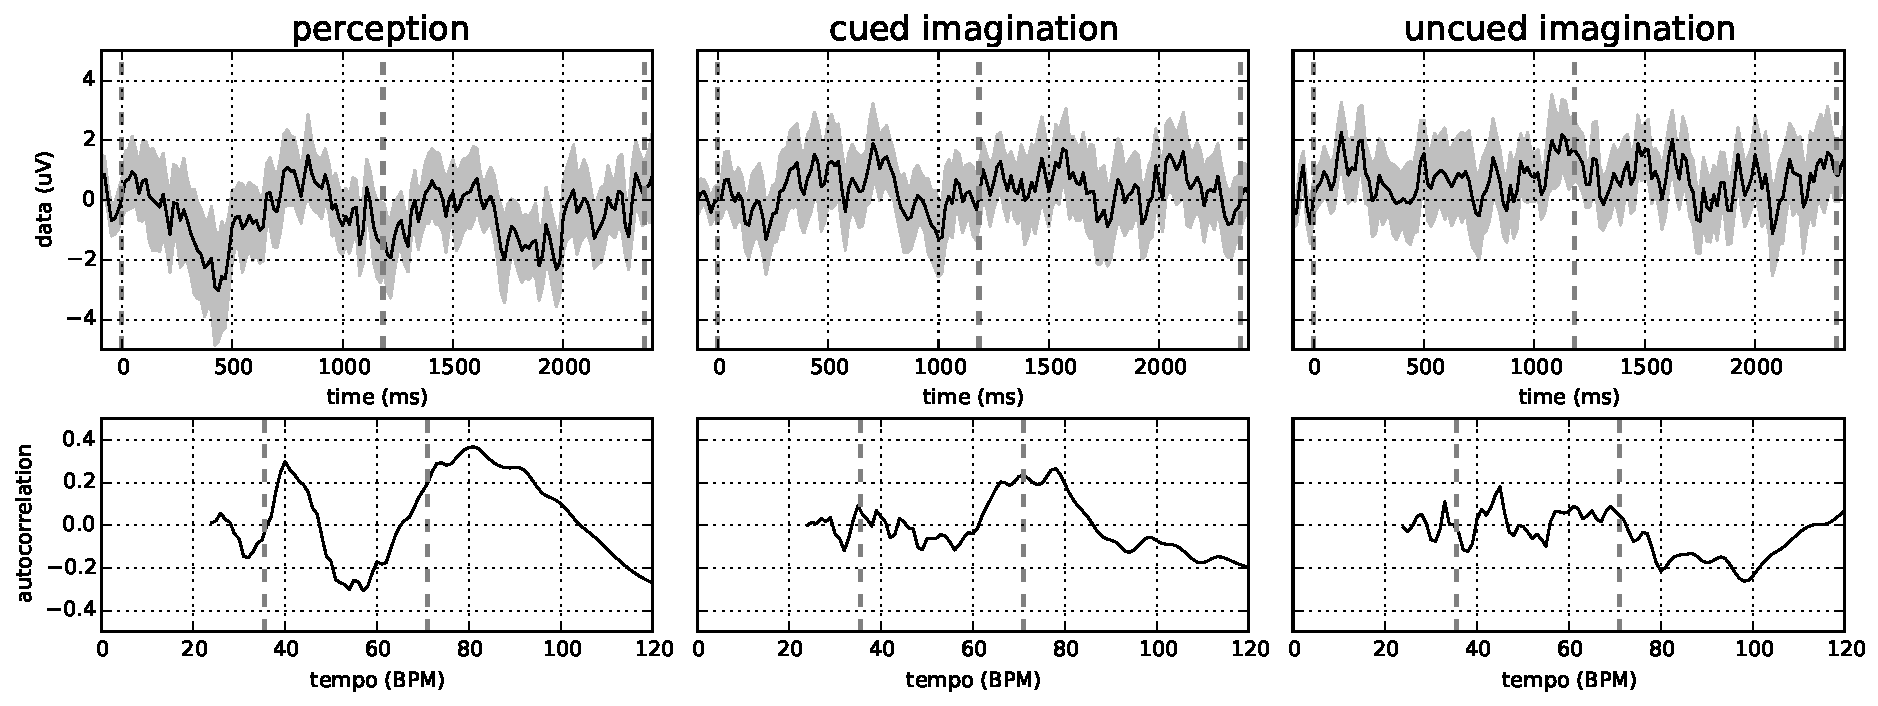
\includegraphics[width=\textwidth,keepaspectratio=true]{Figures/non-overlap_bar-aligned-ERPs.pdf}
%   \\\vspace{-0.8em}
    \caption{%
%\textit{beats are roughly evenly spaced - these peaks are not. looks like onset detection not beat detection. Would cause over-estimation of tempo (makes it seem faster than it is - Jessica)}
Top: Mean and standard deviation over all 64 EEG channels of the bar-aligned ERPs
(without epochs overlap)
for ``Chim Chim Cheree (lyrics)'' in conditions 1--3 for participant P01.
Each ERP was averaged over 25 epochs (5 from each trial).
Bottom: Corresponding autocorrelation scores in the relevant tempo range.
Dashed lines indicate downbeats (top) and the approximate bar tempo of the stimulus plus its lower tempo harmonic (bottom).
%NOTE: downbeat times are based on audio beat detection in stimulus!
}
    \label{fig:non-overlap_bar-aligned-ERPs}
  \end{center}
%  \vspace{-3em}
\end{figure}

In order to analyze this periodicity, we computed the autocorrelation curves by comparing each signal with itself at a range of time lags.
To this end, we aggregated all 64 EEG channels into a mean signal.
We further chose time lags corresponding to the bar tempo range of our stimuli.
The lower end of 24 BPM was determined by our choice of the epoch length. 
Using longer epochs would allow us to extend the tempo range to slower tempi, but this would be at the expense of fewer epochs available for averaging.
%\hl{the following sentence is unclear - slower tempo/bigger epochs} With longer epochs, the tempo range could be extended further towards zero at the expense of fewer epochs available for averaging.

In general, more distinct peaks in the autocorrelation were observed in the perception condition.
For the two imagination conditions, peaks were more blurred as can also be seen in \autoref{fig:non-overlap_bar-aligned-ERPs}.
This is most likely caused by the lack of a time locking mechanism, which allows the tempo to vary.
This hypothesis is also backed by the observation that artificially jittering the bar onsets results in a decrease in autocorrelation.

Most notably, we ensured that the bar-aligned epochs did not overlap by rejecting some of the epochs.
If they overlap, a single data segment can contribute to multiple epochs at different time points.
This can induce misleading autocorrelation peaks that are not supported by the raw data.


\subsection*{Analyzing Single Trials}

With the interesting observations reported in the preceding section, the question arises whether the tempo could similarly be estimated through autocorrelation from single trials. 
Single trial tempo estimation is important for our BCI in order to reduce patient fatigue during use.
Here, we face several challenges. 
First, there are too few bar-aligned epochs in a single trial to use ERPs.
Second, we neither know the tempo of the stimulus nor do we have beat annotations available.
Therefore, there are no reference points for extracting bar-aligned epochs.
Moreover, we wanted to address the problem of possible tempo variance in the imagination conditions.

\autoref{fig:sliding-window-analysis} illustrates our proposed solution to this problem.
We move a 2.5-second sliding window over the mean EEG signal aggregated over all channels.
At each position with a hop size of 5 samples at 64Hz, we compute the autocorrelation curve.
The curves for the individual window segments are stacked into a 2-dimensional matrix with the first dimension corresponding to the window offset in the trial signal and the second dimension corresponding to the possible tempo values.
Hence, each matrix value holds the score for a certain tempo at one specific point in the trial.
The scores in the matrix are finally aggregated deriving an estimated tempo value for the trial.
\autoref{fig:sliding-window-analysis} shows how the mean and maximum values are aggregated over all matrix rows.

\begin{figure}[t]
  \begin{center}
    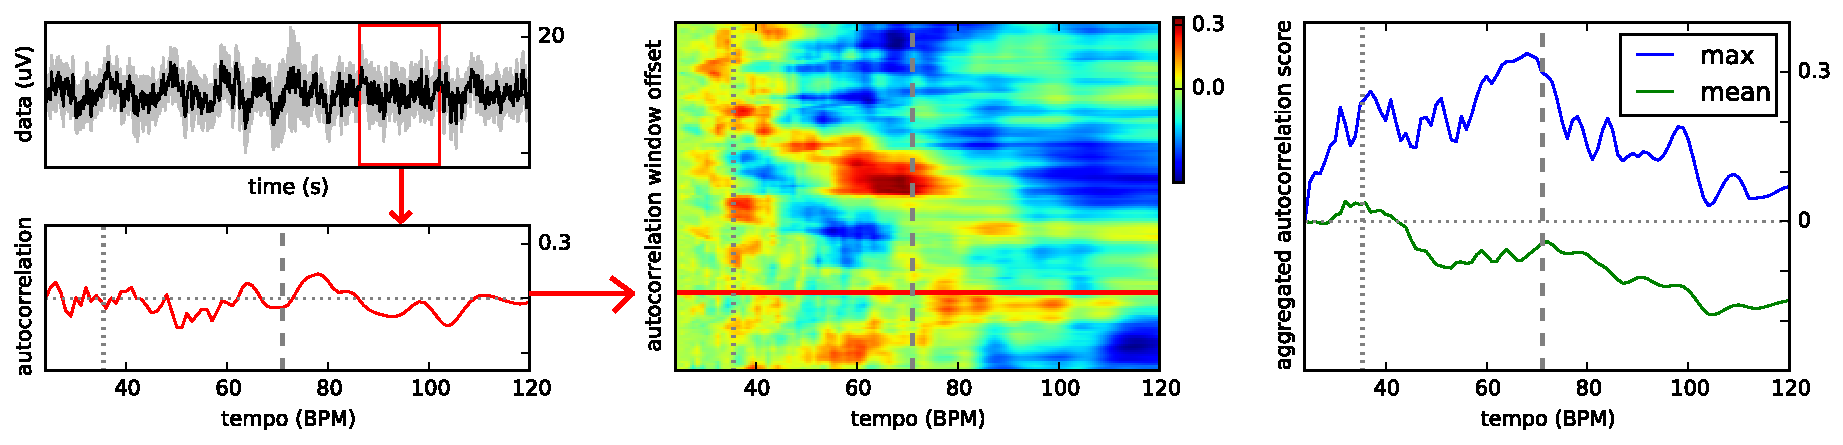
\includegraphics[width=\textwidth,keepaspectratio=true]{Figures/sliding-window-analysis_arrow.pdf}
%    \\\vspace{-0.8em}
    \caption{%
Schema of the proposed tempo estimation technique.
All plots refer to the first of the five trials contributing to the imagination ERP of ``Chim Chim Cheree (lyrics)'' in  \autoref{fig:non-overlap_bar-aligned-ERPs}, middle.
Left top: EEG waveform (mean of all 64 channels) for the whole trial with the red box indicating the sliding window of 2.5 seconds.
Left bottom: Autocorrelation curve for this specific segment of the trial.
Middle: Vertically stacked autocorrelation curves for the whole trial with the red horizontal line indicating the position of the sliding window shown on the left.
Right: Aggregated autocorrelation scores (mean and max) for the whole trial.
Dashed vertical lines indicate the stimulus bar tempo.
Dotted vertical lines refer to half the bar tempo.
    }
    \label{fig:sliding-window-analysis}
  \end{center}
%  \vspace{-2em}
\end{figure}

Ideally, the score for the actual tempo should be stable throughout the whole trial.
However, we observed substantial fluctuation within many trials.
While the mean and maximum over all matrix rows often produce significant peaks in the aggregated autocorrelation curve, the following heuristic has led to slightly more stable results:
\begin{enumerate}
\item
        In each row, find the pair of tempo values with the maximal combined score.
\item
        Select the median of all selected pairs.
\item
        From this pair, return the tempo value with the higher mean value over
all rows.
\end{enumerate}

For the evaluation of our heuristic, we computed the mean absolute error of the estimated tempo and the actual tempo.
We also considered the tempo harmonic below and above the correct value, i.e. half or twice the tempo, as a correct result.
The prediction error, averaged across all stimuli, varied considerably between participants ranging from 7.07, 7.15, and 8.11 in the three conditions for participant P14 up to 9.81, 10.04, and 12.58 for P12.
\autoref{fig:tempo-error-per-stim-cond} summarizes the errors for each stimulus over all trials of all participants.
The figure clearly shows a trend that tempo is easier to predict for some stimuli, such as ``Chim Chim Cheree'' (ID 1 and 11) and ``Mary had a little lamb'' (ID 4 and 14), than for others.
The slowest stimulus, the ``Imperial March'' (ID 23) has the highest variation of prediction accuracy.
Although it is too early to draw definitive conclusions, the data also suggest that single-trial tempo estimation does not depend on the condition (perception or imagination) but rather relies on the tempo of a stimulus.

\begin{figure}
  \begin{center}

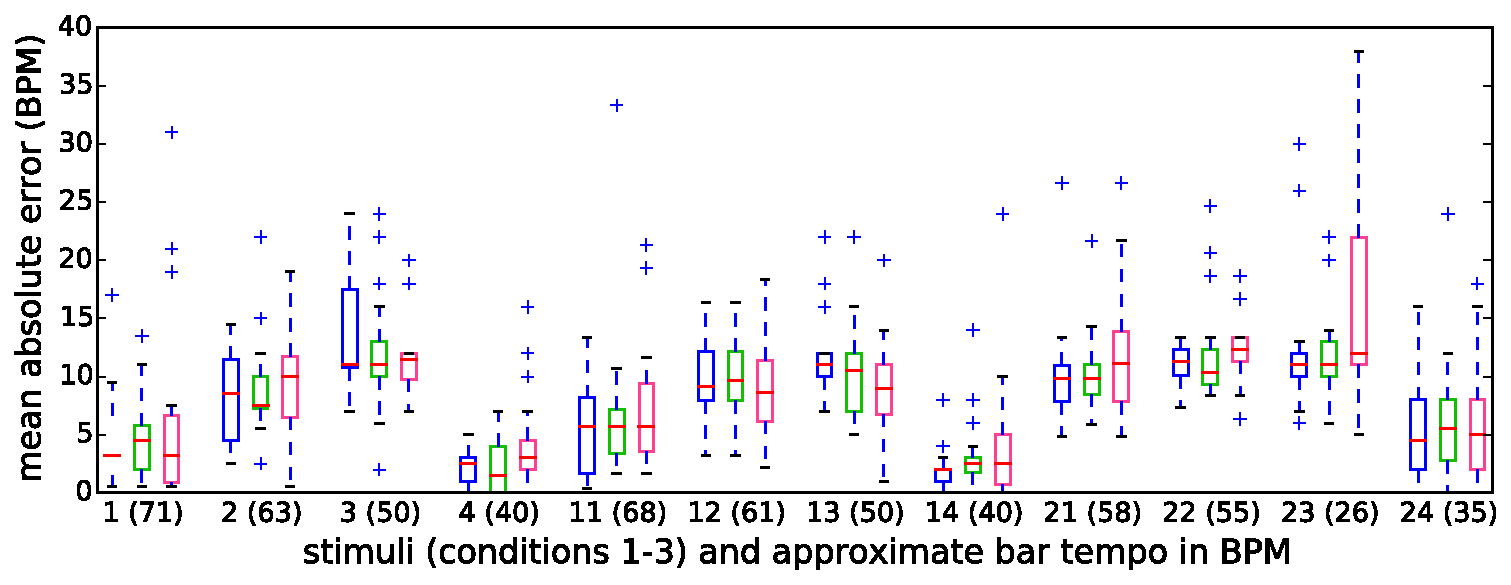
\includegraphics[width=\textwidth,keepaspectratio=true]{Figures/tempo-error-per-stim-cond-all_colour.pdf}
%  \\\vspace{-0.8em}
    \caption{Aggregated errors of single trial tempo prediction over all 5 participants. The true tempo is indicated in brackets with the mean absolute error for each stimulus indicated with a red bar. Each box contains 50\% of the error values for perception (blue), cued imagination (green) and uncued imagination (magenta). The whiskers contain an additional 25\% of the error values. Each cross indicates an outlier. }
    \label{fig:tempo-error-per-stim-cond}
  \end{center}
%  \vspace{-2em}
\end{figure}
